\chapter{The hosted languages}

Poplog's front-ends are not bindings, bridges or embeddings. Each is a
compiler written in Pop-11 that plants code for the same VM, and the result
lives in the same heap as everything else. Switching language switches the
\emph{reader}; it does not switch worlds.

\begin{figure}[H]
\centering
\begin{minipage}[t]{0.485\linewidth}\centering
  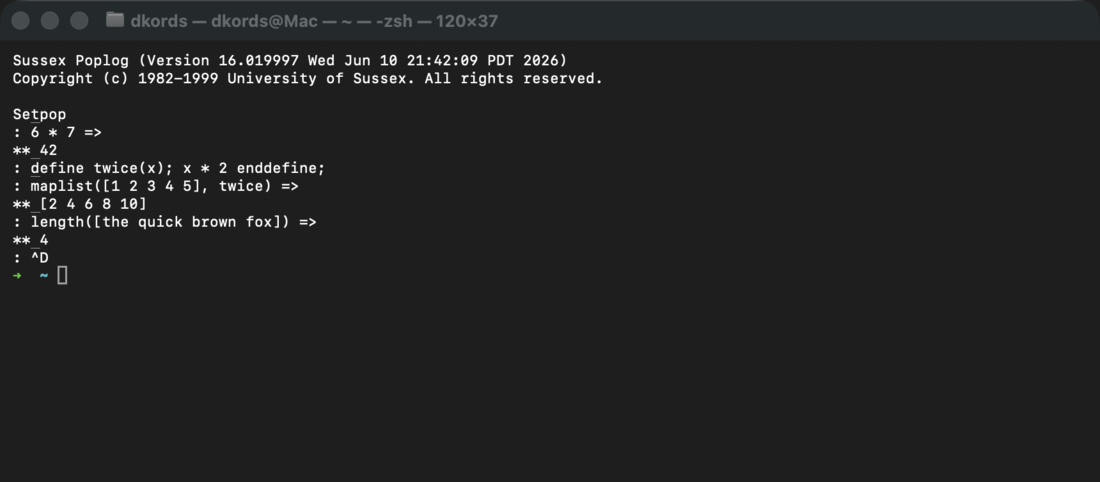
\includegraphics[width=\linewidth]{figures/repl-pop11}\\[3pt]
  {\footnotesize\sffamily\color{popgrey}Pop-11 --- the core language}
\end{minipage}\hfill
\begin{minipage}[t]{0.485\linewidth}\centering
  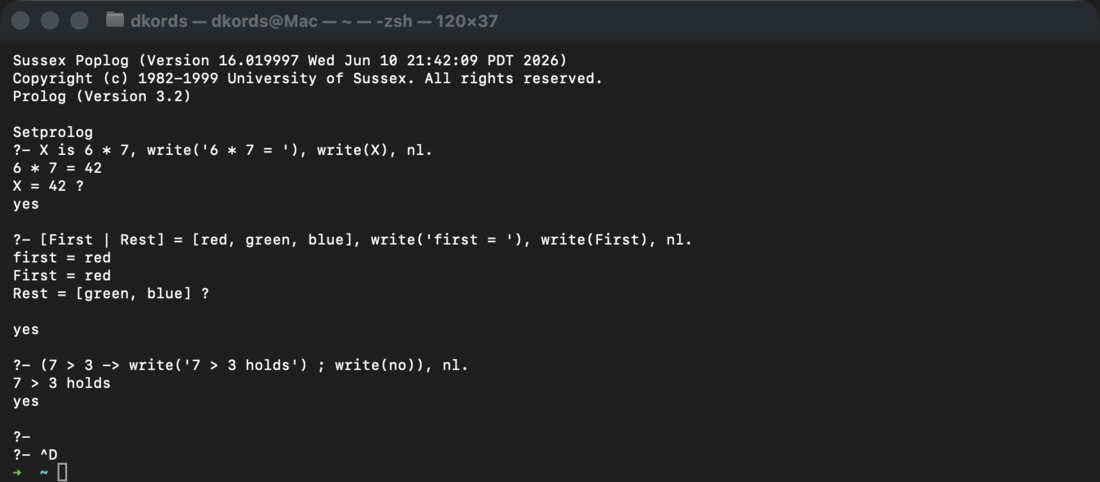
\includegraphics[width=\linewidth]{figures/repl-prolog}\\[3pt]
  {\footnotesize\sffamily\color{popgrey}Prolog --- Edinburgh syntax}
\end{minipage}

\vspace{10pt}
\begin{minipage}[t]{0.485\linewidth}\centering
  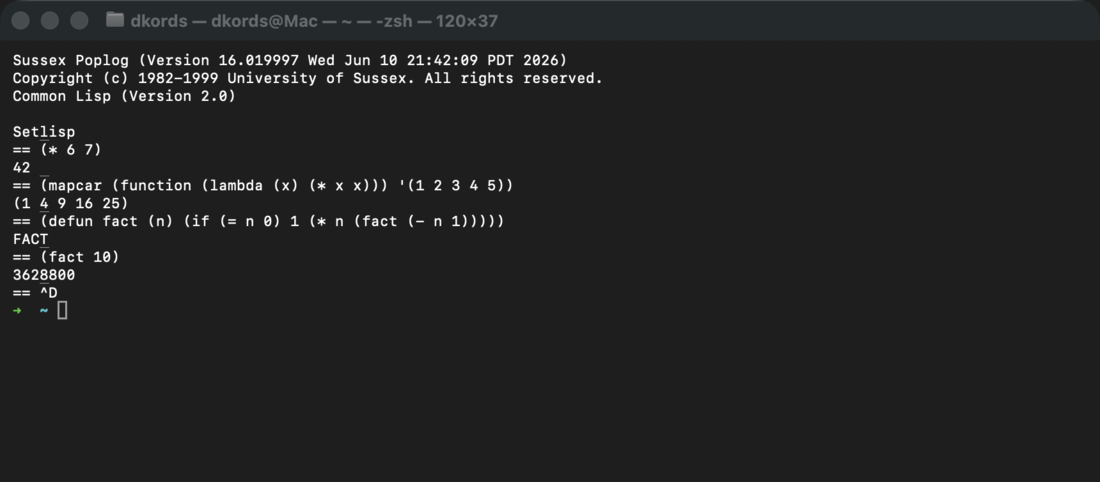
\includegraphics[width=\linewidth]{figures/repl-clisp}\\[3pt]
  {\footnotesize\sffamily\color{popgrey}Common Lisp --- CLTL2}
\end{minipage}\hfill
\begin{minipage}[t]{0.485\linewidth}\centering
  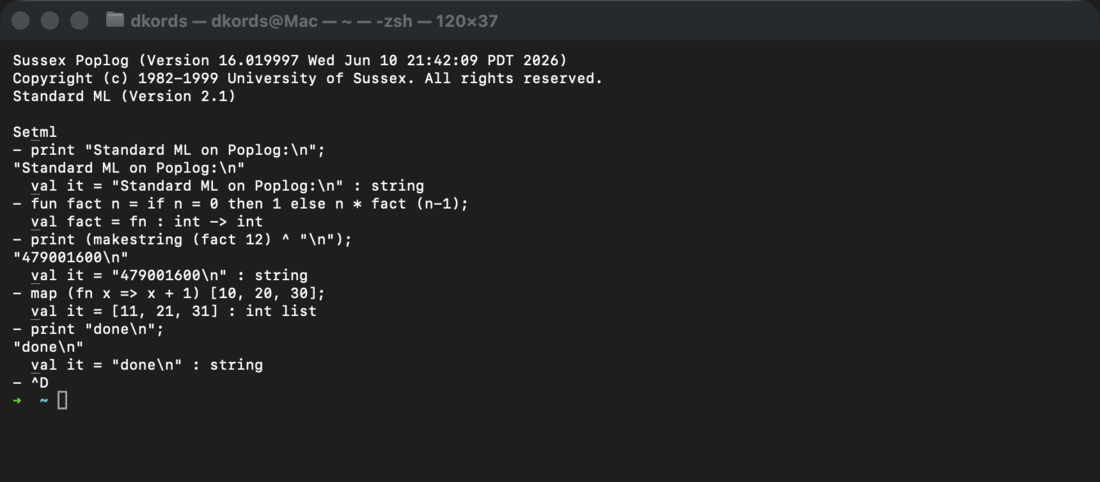
\includegraphics[width=\linewidth]{figures/repl-pml}\\[3pt]
  {\footnotesize\sffamily\color{popgrey}Standard ML --- type inference}
\end{minipage}
\caption*{\small Four front-ends, one engine, one banner --- captured on the
Apple Silicon build. Each image is the same \code{basepop11} with a different
language compiled into it.}
\end{figure}

\section{Prolog}

Edinburgh-syntax Prolog, implemented as 51 Pop-11 files under
\code{pop/plog/src/} --- reader, term representation, unification, clause
store and control. Because it is open Pop-11 rather than a sealed engine,
extending it with new built-ins is an afternoon's work, not a fork.

\begin{lstlisting}[language=PrologX]
parent(tom, ann).
parent(tom, liz).
parent(ann, kim).
grandparent(X, Z) :- parent(X, Y), parent(Y, Z).
ancestor(X, Y)    :- parent(X, Y).
ancestor(X, Z)    :- parent(X, Y), ancestor(Y, Z).
\end{lstlisting}

\begin{repl}
$ ./poplog basepop11 -target/psv/prolog.psv
?- ['fam.pl'].
fam.pl consulted
yes
?- grandparent(tom, W).
W = kim
?- ancestor(tom, W).
W = ann   W = liz   W = kim
?- parent(P, kim).
P = ann
\end{repl}

\begin{callout}{A small surprise}
Poplog's Prolog is deliberately lean: list predicates such as
\code{member/2} and \code{append/3} are \emph{not} built in. Several library
files under \code{pop/plog/lib/} define them, or you write the two clauses
yourself --- which, for a system whose point is that you can see and change
the engine, is in keeping.
\end{callout}

\section{Common Lisp}

Compatible with most of CLTL2. It is a genuine Common Lisp --- packages,
macros, \code{format}, the condition system --- compiled to native code by
the same back-end as everything else.

\begin{lstlisting}[language=Lisp]
(defun sq (x) (* x x))
(print (sq 9))
(print (mapcar (function sq) (list 1 2 3)))
\end{lstlisting}
\begin{repl}
SQ
81
(1 4 9)
\end{repl}

Remember that the reader upcases: \code{sq} and \code{SQ} are the same
symbol, and \code{\#}, \code{.}, \code{,}, \code{@} and \code{:} are reader
macros. \code{help poptolisp} is a translation table for Pop-11 programmers
arriving in Lisp, and \code{help poplisp} documents the mixed-language
interface.

\section{Standard ML}

A full Standard ML with Hindley--Milner type inference, and the strongest
demonstration that the VM is language-agnostic: static typing, pattern-matching
function clauses and polymorphism all sit on the same dynamically typed heap.

\begin{lstlisting}[language=SML]
fun sq (x:int) = x * x;
map sq [1,2,3];
fun fact 0 = 1 | fact n = n * fact(n-1);
fact 10;
\end{lstlisting}
\begin{repl}
  val sq = fn : int -> int
  val it = [1, 4, 9] : int list
  val fact = fn : int -> int
  val it = 3628800 : int
\end{repl}

The type-checker is where ML's surprises live rather than the runtime: an
unannotated \code{fun sq x = x * x} is rejected, because \code{*} is
overloaded and there is nothing to resolve it against.

\section{Forth}

Those three, with Pop-11 itself, are classic Poplog. This fork adds a fifth, and it
is the shortest route to understanding why hosting on the VM is cheap:
\textbf{Forth's data stack is the Poplog user stack.} A Forth primitive is an
ordinary open-stack Pop-11 procedure --- \code{+} is
\code{define f\_plus(x,y); x+y enddefine} --- and no data structure is
interposed at all.

Colon definitions are not threaded code. \code{: name \ldots ;} is
transpiled to a Pop-11 procedure and run through the incremental compiler, so
a Forth word is a real native procedure; \code{if/else/then},
\code{begin/until}, \code{begin/while/repeat}, \code{do/loop},
\code{recurse} and \code{exit} map onto Pop-11 constructs at compile time.

\begin{lstlisting}[language=Forth]
: sq  dup * ;
9 sq .
: fib  dup 2 < if drop 1 else dup 1 - recurse swap 2 - recurse + then ;
20 fib .
: stars  0 do 42 emit loop ;
10 stars cr
variable acc   5 acc !   acc @ .
\end{lstlisting}
\begin{repl}
$ tools/forth.sh
Poplog Forth.  words / testbench / bye
81  ok
10946  ok
**********
 ok
5  ok
forth> testbench
21 passed, 0 failed   ALL OK   (0.273 ms)
\end{repl}

The core covers arithmetic, about forty stack, comparison, bitwise and I/O
words, native colon definitions, the control words above, counted loops with
\code{i}/\code{j}/\code{leave}, \code{variable}/\code{constant}/\code{@}/\code{!},
a return stack (\code{>r r@ r>}), and string literals. It is younger and
leaner than the mature four --- no \code{+loop}, \code{create does>} or
\code{value} yet, and it is case-sensitive. Because it is pure Pop-11 it runs
on every platform Poplog does; the built-in \code{testbench} is 21/21 on both
macOS \code{arm64} and RISC-V. Implementation:
\code{pop/forth/src/forth.p}, 523 lines.

\section{Crossing between them}

All five share one image, so crossing is a change of reader, not a marshalling
boundary.

\textbf{From any language back to Pop-11}, type \code{pop11}:

\begin{repl}
$ ./poplog basepop11 -target/psv/clisp.psv
(print (* 6 7))
42
pop11
: [a b c] <> [d] =>
** [a b c d]
\end{repl}

\begin{repl}
$ ./poplog basepop11 +target/psv/pml.psv
val x = 6 * 7;
  val x = 42 : int
pop11
: [a b c] <> [d] =>
** [a b c d]
\end{repl}

\textbf{From Pop-11 into Prolog}, the syntax word \code{?-} runs a goal
inline, against the same clause store:

\begin{repl}
: vars greeting = [hello there];
: ?- write(from_prolog), nl.
from_prolog
yes
: rev(greeting) =>
** [there hello]
\end{repl}

\textbf{Defining Prolog predicates in Pop-11} is a documented form
(\code{help define\_prolog}) --- useful when a predicate wants a data
structure or an I/O facility that is easier to reach from Pop-11:

\begin{pop}
define :prolog hello/0(contn);
    lvars contn;
    printf('Hello world\n');
    chain(contn);            ;;; call the continuation = succeed
enddefine;
\end{pop}
\begin{repl}
?- hello.
Hello world
yes
\end{repl}

The continuation-passing shape is not incidental: it is how Poplog's Prolog
represents ``and then carry on solving'', so a Pop-11 predicate that calls
\code{chain(contn)} succeeds once, and one that calls it in a loop is a
generator with backtracking.

\begin{callout}{Which image has which language}
Each shipped image contains the languages compiled into it. \code{prolog.psv}
has Pop-11 and Prolog; \code{clisp.psv} has Pop-11 and Common Lisp;
\code{pml.psv} has Pop-11 and ML. Forth is pure library code --- \code{uses
forth} works anywhere. To get several at once, build an image that loads
them, exactly as \code{make} builds these.
\end{callout}
